\title{Východní Evropa}
\documentclass[10pt,a4paper]{article}
\usepackage[utf8]{inputenc}
\usepackage[czech]{babel}
\usepackage{amsmath}
\usepackage{amsfonts}
\usepackage{amssymb}
\usepackage{chemfig}
\usepackage{geometry}
\usepackage{wrapfig}
\usepackage{graphicx}
\usepackage{floatflt}
\usepackage{hyperref}
\usepackage{fancyhdr}
\usepackage{tabularx}
\usepackage{makecell}
\usepackage{csquotes}
\usepackage{footnote}
\usepackage{movie15}
\MakeOuterQuote{"}

\renewcommand{\labelitemii}{$\circ$}
\renewcommand{\labelitemiii}{--}
\newcommand{\ra}{$\rightarrow$ }
\newcommand{\x}{$\times$ }
\newcommand{\lp}[2]{#1 -- #2}
\newcommand{\timeline}{\input{timeline}}


\geometry{lmargin = 0.8in, rmargin = 0.8in, tmargin = 0.8in, bmargin = 0.8in}
\date{\today}
\author{Jakub Rádl}

\makeatletter
\let\thetitle\@title
\let\theauthor\@author
\makeatother

\hypersetup{
colorlinks=true,
linkcolor=black,
urlcolor=cyan,
}



\begin{document}
\maketitle
\tableofcontents
\begin{figure}[b]
Toto dílo \textit{\thetitle} podléhá licenci Creative Commons \href{https://creativecommons.org/licenses/by-nc/4.0/}{CC BY-NC 4.0}.\\ (creativecommons.org/licenses/by-nc/4.0/)
\end{figure}
\newpage

\newpage
\mbox{}
\vspace{-1.5cm}
\begin{wrapfigure}{r}{4cm}
\frame{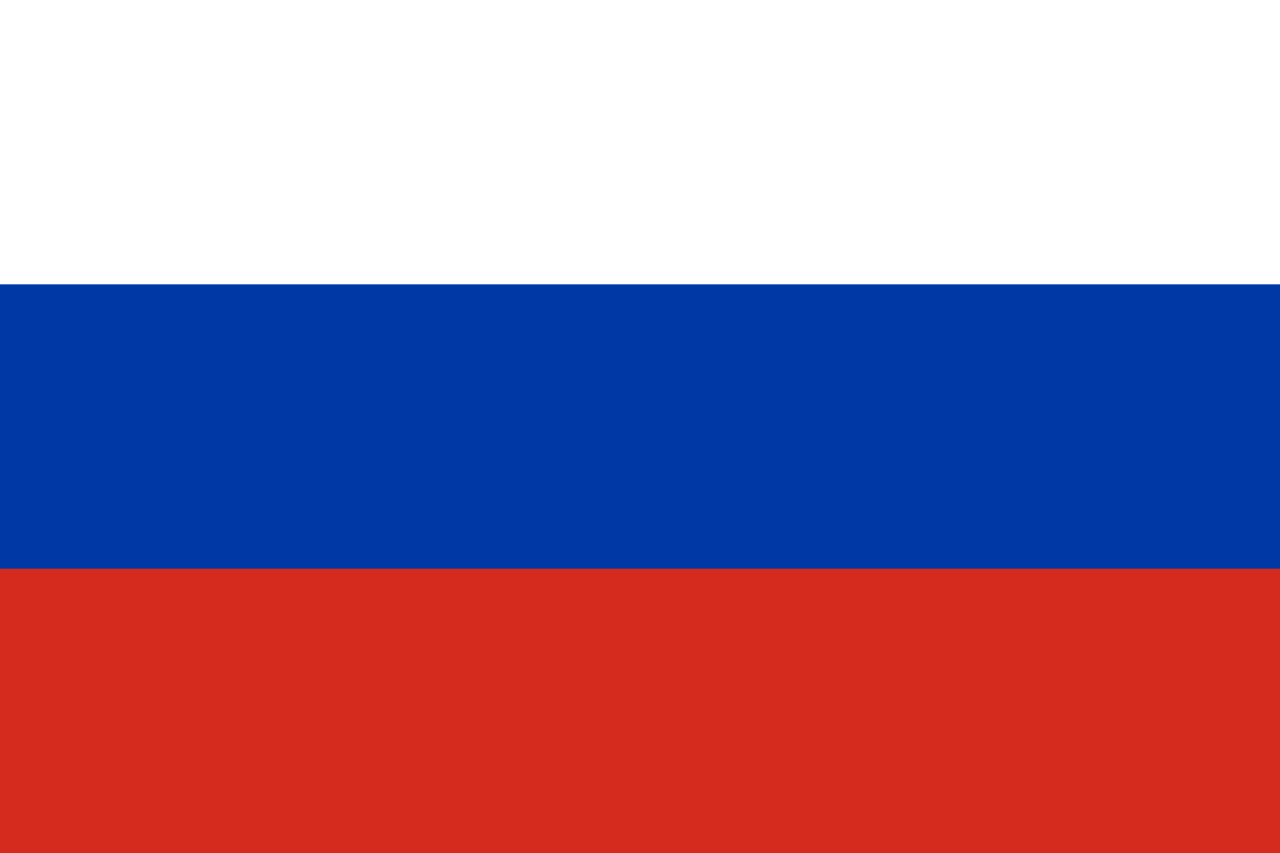
\includegraphics[height=2cm]{pictures/flag_RU.png}}
\vspace{-20pt}
\end{wrapfigure}	
\section{Rusko}
\begin{enumerate}
\item Vyhledej v atlase: Valdajská vrchovina, Středosibiřská vysočina; Kaspická, Severosibiřská nížina, Východoevropská, Západosibiřská rovina; pouště Karakum, Kyzylkum, Pamír, Ťan-Šan, Altaj; poloostrovy Tajmyr, Čukotka, Kamčatka; jezera Aralské, Balchaš, Bajkal, Ladožské, Oněžské; řeky Ob, Syrdarja, Amudarja, Irtyš, Jenisej,Angara, Lena, Amur
\item Co víš o Společenství nezávislých států?
\item Do kterých podnebných pásů zasahuje Rusko?
\item Vyhledej na mapě největší pohoří, nížiny, řeky, jezera v Rusku.
\end{enumerate}

\subsection{Společenství nezávislých států}
\begin{itemize}
\item vznik 1991 jako volný svazek postsovětských států
\item nástupce rozpadlého Sovětského svazu
\item sídlo v Minsku
\item 9 členů, pobaltské státy odmítly vstoupit
\item Turkmenistán je přidružený člen, Ukrajina a Gruzie vystoupili
\item vazba na Rusko
\item koordinace společných obchodní, finančních a bezpečnostních otázek
\end{itemize}

\subsection{Základní informace}
\begin{itemize}
\item počet obyvatel:
\item rozloha: 
\end{itemize}

\subsection{Historie}
\begin{itemize}
\item původně vládne car
\item 1917 -- Bolševická revoluce, nastolení komunistické diktatury s centrálně řízenou ekonomikou
\item 1922 -- vznik SSSR (Svaz Sovětských Socialistických Republik)
\item likvidace odpůrců režimu v koncentračních táborech (gulag), pronásledování inteligence, násilné přemisťování obyvatelstvo
\item po 2. sv. válce ovládnutí komunistického bloku
\item 1991 rozpad SSSR na 15 samostatných států, vznik SNS
\end{itemize}

\paragraph{Sociální prostředí}
\begin{itemize}
\item nerovnoměrné rozmístění obyvatel
\item multietnický stát (Jakuti, Evenkové, Něnci)
\item vylidňování venkova a odlehlých oblastí
\item administrativní členění na 8 okruhů, 22 republik s vládami a parlamenty, oblasti, kraje, autonomní okruhy (Něnci, Evenkové, Jakuti)
\end{itemize}

\subsection{Ekonomika}
\paragraph{Hospodářství}
\begin{itemize}
\item rozsáhlé zásoby narostných surovin, ale nerovnoměrně rozmístěné a na Sibiři obtížně dobyvatelné
\item obrovské dopravní vzdálenosti, zastaralá a nedostatečná dopravní síť, která pokrývá jen část území
	\begin{itemize}
	\item dominance železniční dopravy
	\end{itemize}
\item většina hospodářského potenciálu v evropské části
\item rozsáhlý, ale zastaralý těžký průmysl, není konkurence schopný ostatním státům
\item nízká úroveň spotřebního průmyslu
\item velký význam zbrojního průmyslu
	\begin{itemize}
	\item závod mezi Ruskem a USA
	\item vypovězení smlouvy mezi USA a Ruskem o nepoužívání raket středního doletu v Evropě
	\end{itemize}
\item značné sociální rozdíly mezi Evropou a východem
\item slabé zapojení do světového trhu
	\begin{itemize}
	\item vývoz: ropa, zemní plyn, rudy, uhlí
	\item dovoz: spotřební zboží
	\item Rusko tímto splňuje charakteristiky rozvojových zemí a málo zisků z vývozu investuje do rozvoje ekonomiky
	\item v poslední době nízké ceny ropy
	\item po anexi Krymu sankce \ra zákaz dovozu některého zboží
	\end{itemize}
\item 
\end{itemize}

\paragraph{Hlavní ekonomické regiony}
\begin{itemize}
\item Moskva
\item st. Petersburg
\item Povolží
\item j. Ural
\item Kavkaz
\item Chanty - Mansijsk
\end{itemize}


\end{document}

